\documentclass[12pt,a4paper]{article}

\usepackage{tikz}
\usepackage{incgraph}
\usepackage{hyperref}

\usetikzlibrary{mindmap,shadows}

\begin{document}
\begin{inctext}
    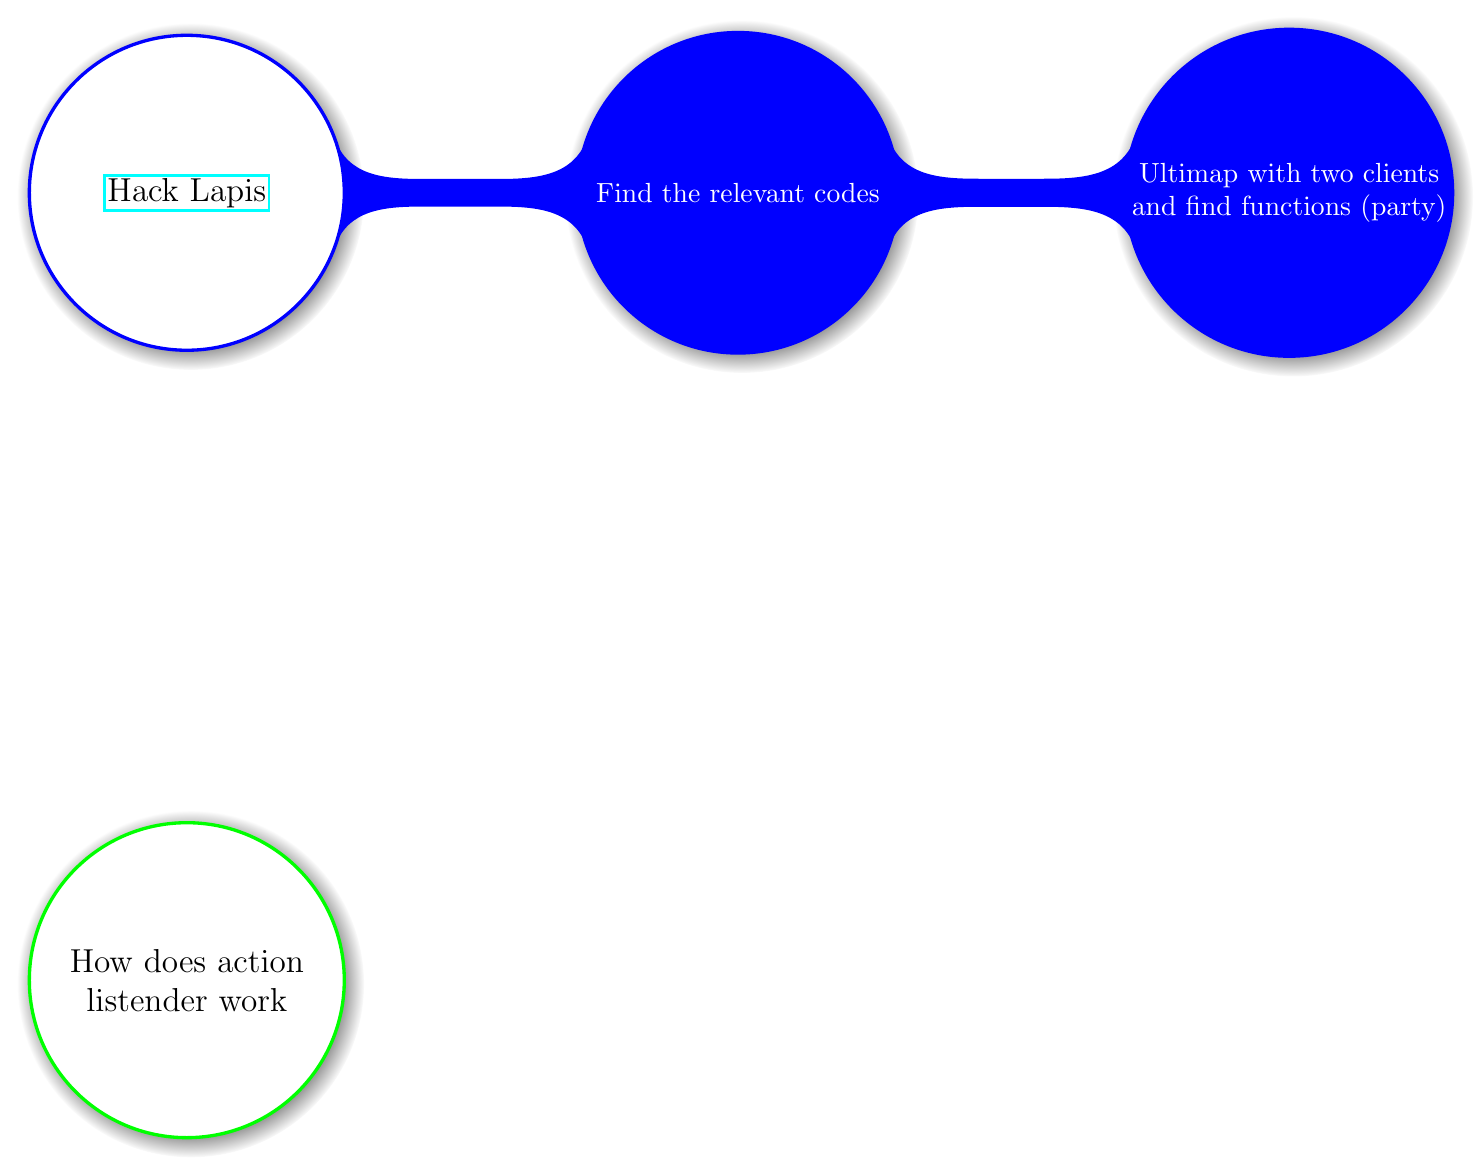
\begin{tikzpicture}[
            mindmap,
            grow cyclic,
            every node/.append style={concept,circular drop shadow, text width=4cm},
            every child/.append style={level distance=7cm, font=\fontsize{10pt}{12pt}},
        ]
        \begin{scope}[
                % lapis
                concept color=blue,
                every child/.append style={color=white}
            ]
            \node[root concept, fill=white](lapis){
                \href{https://lapis.mgame.com/}{Hack Lapis}
            }
            child {
                    node{
                            \href{}{Find the relevant codes}
                        }
                    child{
                            node{
                                    Ultimap with two clients and find functions (party)
                                }
                        }
                }
            ;
        \end{scope}

        \begin{scope}[
                concept color=green,
                % every child/.append style={color=white}
            ]
            \node[root concept, fill=white, yshift=-10cm](actionlistender){
                \href{}{How does action listender work}
            };
        \end{scope}
    \end{tikzpicture}
\end{inctext}
\end{document}